\documentclass{beamer}

\mode<presentation>
{
  \usetheme{default}
  % or ...

  \setbeamercovered{transparent}
  % or whatever (possibly just delete it)
}


\usepackage[english]{babel}
\usepackage[latin1]{inputenc}
\usepackage{graphicx}
\usepackage{fancyvrb}
\usepackage[T1]{fontenc}
\fontencoding{T1}\selectfont
%\usepackage{verbatim}

%\usepackage{helvet}
%\renewcommand\familydefault{\sfdefault}

\usepackage{amsmath,amsfonts,amssymb}
\newcommand{\bsym}{\boldsymbol}
\newcommand{\eps}{\varepsilon}
\newcommand{\bx}{\mathbf{x}}
\newcommand{\bX}{\mathbf{X}}
\newcommand{\bZ}{\mathbf{Z}}
\newcommand{\bz}{\mathbf{z}}
\newcommand{\code}{\texttt}
\newcommand{\wh}{\widehat}
\newcommand{\R}{\textsf{R}}
\newcommand{\pkg}{\textbf}

\title[Methods for Reproducible Research]{Tutorial: Methods for
  Reproducible Research}

\author{Roger D. Peng\inst{}}

\institute{
  %\inst{1}%
  Department Biostatistics\\
  Johns Hopkins Bloomberg School of Public Health
}

\date[ENAR 2009]{ENAR 2009}





\usepackage{Sweave}
\begin{document}

\begin{frame}
\maketitle
\end{frame}


\begin{frame}{Replication}
  The ultimate standard for strengthening scientific evidence is
  \textbf{replication} of findings and studies with independent
\begin{itemize}
\item multiple investigators
\item data
\item analytical methods
\item laboratories
\item instruments
\end{itemize}
Replication is particularly important in studies that can impact broad
policy or regulatory decisions.
\end{frame}

\begin{frame}{Reproducible Research}
  Why do we need reproducible research?
  \begin{itemize}
    \item Many studies cannot be replicated
      \begin{itemize}
      \item No time
      \item No money
      \item Unique
      \end{itemize}
    \item New technologies increasing data collection throughput; data
      are more complex and extremely high dimensional
    \item Existing databases can be merged into new ``megadatabases''
    \item Computing power is greatly increased, allowing more
      sophisticated analyses
    \item For every field ``$X$'' there is a field ``Computational X''
      (de~Leeuw's Law)
  \end{itemize}  
\end{frame}

\begin{frame}{Reproducible Research}
  
  Today, scientific papers published in journals represent the
  \textbf{advertising} of the research (Claerbout)

\end{frame}  


\begin{frame}{Research Pipeline: Model for Reproducible Research}
  \begin{center}
    \includegraphics[width=4.2in]{pipeline}
  \end{center}
\end{frame}


\begin{frame}{Reproducible Research}
  What is this reproducible research?
  \begin{itemize}
    \item Analytic data are available
    \item Analytic code are available
    \item Documentation of code and data
    \item Standard means of distribution
  \end{itemize}
\end{frame}

\begin{frame}{Who are the Players?}
Authors
\begin{itemize}
\item Want to make their research reproducible
\item Want tools for RR to make their lives easier (or at least not
  much harder)
\end{itemize}
Readers
\begin{itemize}
\item Want to reproduce (and perhaps expand upon) interesting findings
\item Want tools for RR to make their lives easier
\end{itemize}
\end{frame}

\begin{frame}{Theory...}
\begin{center}
  \includegraphics[width=4.2in]{ajesnapshot}
\end{center}
\end{frame}
  
\begin{frame}{...Methods?}
Authors
\begin{itemize}
\item Just put stuff on the web
\item Journal supplementary materials
\item There are some central databases for various fields (e.g. biology, ICPSR)
\end{itemize}
Readers
\begin{itemize}
\item Just download the data and figure it out
\item Get the software and run it
\end{itemize}  
\end{frame}
  

\begin{frame}{Problems}
  Even in the best of cases
  \begin{itemize}
  \item Authors must undertake considerable effort to put data/results
    on the web (may not have resource like a webserver)
  \item Readers must download data/results individually and piece together which data go with which code sections, etc.
  \item Authors/readers must manually interact with websites
  \item There is no \textbf{single document} to integrate data
    analysis with textual representations; i.e. data, code, and text
    are not linked
  \end{itemize}
\end{frame}

\begin{frame}{Literate Programming}
  The idea of a literate program comes from Don Knuth:
\begin{itemize}
\item An article is a stream of \textbf{text} and \textbf{code}
\item Analysis code is divided into text and code ``chunks''
\item Each code chunk loads data and computes results
\item Presentation code formats results (tables, figures, etc.)
\item Article text explains what is going on
\item Literate programs can be \textbf{weaved} to produce
  human-readable documents and \textbf{tangled} to produce
  machine-readable documents
  \end{itemize}
\end{frame}

\begin{frame}{Literate Programming}
Literate programming is a general concept. We need
\begin{enumerate}
\item A documentation language (human readable)
\item A programming language (machine readable)
\end{enumerate}
We will be using \LaTeX\ and \R\ as our documentation and programming
languages.
\begin{itemize}
\item The system implementing the necessary machinery is called
\textbf{Sweave}, developed by Friedrich Leisch (member of the R Core)
\item Main web site: http://www.statistik.lmu.de/\~{}leisch/Sweave/
\end{itemize}
Alternatives to \LaTeX/\R\ exist, suchas HTML/\R\ (package
\textbf{R2HTML}) and ODF/\R\ (package \textbf{odfWeave}).
\end{frame}

\begin{frame}[fragile]{Example of Literate Programming}
I want to calculate the current time in \R.
\begin{Schunk}
\begin{Sinput}
> time <- format(Sys.time(), "%a %b %d %X %Y")
\end{Sinput}
\end{Schunk}
The current time is Mon Mar 16 16:52:53 2009.  The text and \R\ code are
interwoven:
\begin{verbatim}
  The time is Mon Mar 16 16:52:53 2009
\end{verbatim}
Papers, dissertations, and presentations can be written using literate
programming.
\end{frame}

\begin{frame}{Example of Literate Programming}
  Even books can be written!
  \begin{center}
    \includegraphics[width=4in]{coverback}
    \end{center}
  \end{frame}

\begin{frame}{Literate Programming: Pros and Cons}
Advantages of switching to literate programming
\begin{itemize}
\item Text and code all in one place, in logical order
\item Data, results automatically updated to reflect external changes
\item Automatic ``regression test'' when building document
\end{itemize}
Some disadvantages
\begin{itemize}
\item Text and code all in one place; can make \LaTeX\ difficult to
  read sometimes, especially if there is \textbf{a lot} of code
\item Can substantially slow down the processing of documents
  (although there are some tools to help there)
\end{itemize}
The \textbf{make} tool can be of great help but we will not discuss
that here.
\end{frame}

\begin{frame}{Sweave}
What is Sweave?
\begin{itemize}
\item Sweave is a function and also a command-line script that comes
  with R (it is part of the \pkg{utils} package)
\item The function can be invoked as \code{Sweave()}
\item The command-line script is in the form \code{R CMD Sweave}
\end{itemize}
There is also Stangle
\begin{itemize}
\item \code{Stangle()}
\item \code{R CMD Stangle}
\end{itemize}
But one thing at a time....
\end{frame}


\begin{frame}[fragile]{Basic Sweave Document: \code{example.Rnw}}
  \begin{Verbatim}
    \documentclass[11pt]{article}
    \title{My First Sweave Document}
    \begin{document}
    \maketitle

    This is some text (i.e. a ``text chunk'').   

    Here is a code chunk
    <<>>=
    set.seed(1)
    x <- rnorm(100)
    mean(x)
    @
    \end{document}
  \end{Verbatim}
\end{frame}

\begin{frame}[fragile]{Processing a Sweave Document}
\begin{Verbatim}  
  ## create 'example.tex'
  ## In R
  library(utils)
  Sweave("example.Rnw")

  ## On the command line
  R CMD Sweave example.Rnw
  
  ## Usual LaTeX processing
  ## One of the following will work
  texi2dvi example.tex  ## Create DVI file
  latex example.tex
  texi2dvi --pdf example.tex  ## Create PDF file
  pdflatex example.tex
  \end{Verbatim}
\end{frame}

\begin{frame}[fragile]{What \code{R CMD Sweave} Produces: \code{example.tex}}
\begin{Verbatim}
\documentclass[11pt]{article}
\title{My First Sweave Document}
\usepackage{Sweave}
\begin{document}
\maketitle
This is some text (i.e. a ``text chunk'').
Here is a code chunk
\begin{Schunk}
\begin{Sinput}
> set.seed(1)
> x <- rnorm(100)
> mean(x)
\end{Sinput}
\begin{Soutput}
[1] 0.1088874
\end{Soutput}
\end{Schunk}
\end{document}
\end{Verbatim}
\end{frame}

\begin{frame}{The Resulting PDF Document}
  \begin{center}
    \includegraphics{examplepdf}
  \end{center}
\end{frame}

\begin{frame}[fragile]{A Few Good Notes}
Code chunks begin with
\begin{Verbatim}
<<>>=
\end{Verbatim}
and end with
\begin{Verbatim}
@
\end{Verbatim}
All R code goes in between.\\[1em]

Code chunks can have \textbf{names}, which is useful when we start
making graphics (more later).
\begin{Verbatim}
<<loaddata>>=
## R code goes here
@
\end{Verbatim}
By default, the code in a code chunk will be \textbf{echo}ed, as will
the results of the computation (if there is something to print).
\end{frame}

\begin{frame}{Note on Processing Sweave Documents}
It's important to remember that the order is
\begin{enumerate}
\item example.Rnw
\item example.tex
\item example.pdf
\end{enumerate}
The \code{.tex} file is not something that we care about and
\textbf{should not edit} (always edit the \code{.Rnw} file). It is
merely an intermediary between the Sweave document and the PDF.
\end{frame}



\begin{frame}[fragile]{Basic Sweave Document: \code{example2.Rnw}}
  \begin{Verbatim}
    \documentclass[11pt]{article}
    \title{My First Sweave Document}
    \author{Roger D. Peng}
    \begin{document}
    \maketitle
    \section{Introduction}
    This is some text (i.e. a ``text chunk'').   
    Here is a code chunk
    <<simulation,echo=false>>=
    set.seed(1)
    x <- rnorm(100)
    mean(x)
    @
    \end{document}
  \end{Verbatim}
\end{frame}

\begin{frame}{Result}
  \begin{center}
    \includegraphics{example2pdf}
  \end{center}
\end{frame}

\begin{frame}[fragile]{Basic Sweave Document: \code{example3.Rnw}}
\begin{Verbatim}
  \documentclass[11pt]{article}
  \title{My First Sweave Document}
  \begin{document}
  \maketitle
  
  \section{Introduction}
  This is some text (i.e. a ``text chunk'').   
  Here is a code chunk but it doesn't print anything!
  <<simulation,echo=false,results=hide>>=
  x <- rnorm(100); y <- x + rnorm(100, sd = 0.5)
  mean(x)
  @
  \end{document}
\end{Verbatim}
\end{frame}

\begin{frame}{Result}
  \begin{center}
    \includegraphics{example3pdf}
  \end{center}
\end{frame}


\begin{frame}[fragile]{Inline Text: \code{example4.Rnw}}    
  \begin{Verbatim}
  \documentclass[11pt]{article}
  \begin{document}
  \section{Introduction}
  
  <<computetime,echo=false>>=
  time <- format(Sys.time(), "%a %b %d %X %Y")
  rand <- rnorm(1)
  @
  The current time is \Sexpr{time}. My favorite random
  number is \Sexpr{rand}.
  \end{document}
\end{Verbatim}
\end{frame}

\begin{frame}{Inline Text}
  \begin{center}
    \includegraphics{example4pdf}
  \end{center}
\end{frame}

\begin{frame}[fragile]{Graphics: \code{example5.Rnw}}
\begin{Verbatim}
  \documentclass[11pt]{article}
  \begin{document}
  \section{Introduction}
  Let's first simulate some data.
  <<computetime,echo=true>>=
  x <- rnorm(100); y <- x + rnorm(100, sd = 0.5)
  @
  Here is a scatterplot of the data.
  <<scatterplot,fig=true,width=8,height=4>>=
  par(mar = c(5, 4, 1, 1), las = 1)
  plot(x, y, main = "My Data")
  @
  \end{document}
\end{Verbatim}
\end{frame}

\begin{frame}[fragile]{What Sweave Produces}
\begin{Verbatim}
\documentclass[11pt]{article}
\usepackage{Sweave}

\begin{document}

\section{Introduction}
Let's first simulate some data.
\begin{Schunk}
\begin{Sinput}
> x <- rnorm(100)
> y <- x + rnorm(100, sd = 0.5)
\end{Sinput}
\end{Schunk}
\end{Verbatim}
\end{frame}

\begin{frame}[fragile]{What Sweave Produces (cont'd)}
\begin{Verbatim}
Here is a scatterplot of the data.
\begin{Schunk}
\begin{Sinput}
> par(mar = c(5, 4, 1, 1), las = 1)
> plot(x, y, main = "My Data")
\end{Sinput}
\end{Schunk}

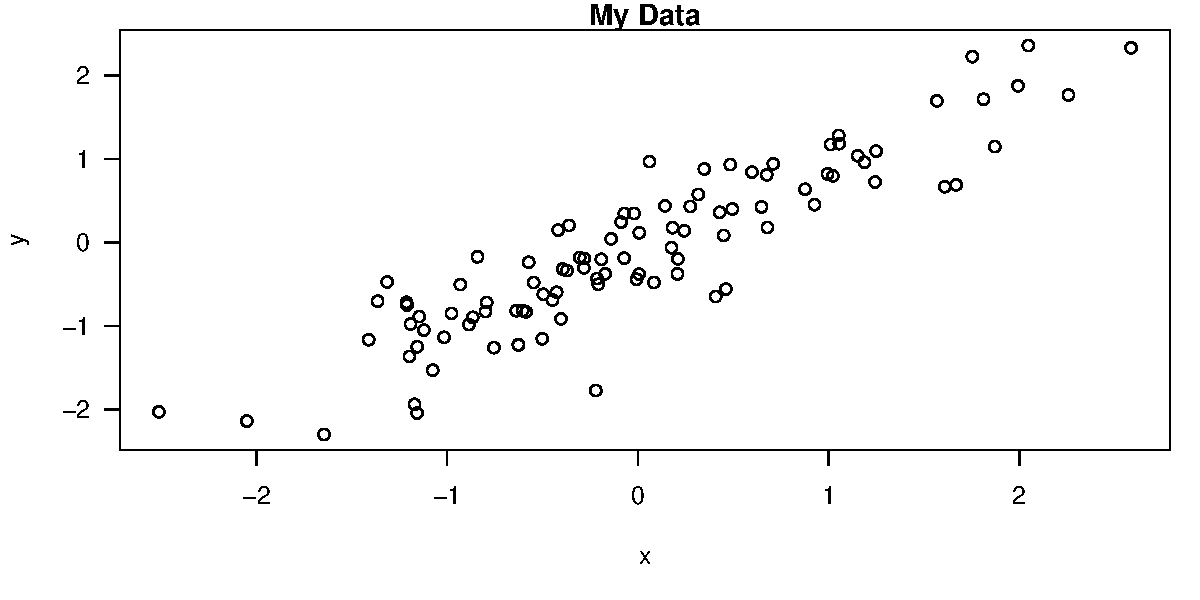
\includegraphics{example5-scatterplot}

\end{document}
\end{Verbatim}
\end{frame}

\begin{frame}{Graphics}
  \begin{center}
    \includegraphics{example5pdf}
  \end{center}
\end{frame}

\begin{frame}[fragile]{Figures}
\begin{Verbatim}
\documentclass[11pt]{article}

\begin{document}
\section{Introduction}

Let's first simulate some data.

<<simulation,echo=true>>=
x <- rnorm(100); y <- x + rnorm(100, sd = 0.5)
@
\end{Verbatim}
\end{frame}

\begin{frame}[fragile]{Figures (cont'd)}
\begin{Verbatim}
Figure~\ref{plot} shows a scatterplot of the data.

\begin{figure}  
<<scatterplot,fig=true,width=8,height=4>>=
par(mar = c(5, 4, 1, 1), las = 1)
plot(x, y, main = "My Data")
@
\caption{Scatterplot}
\label{plot}  
\end{figure}  

\end{document}
\end{Verbatim}
\end{frame}

\begin{frame}[fragile]{Getting the Code Out}
  Sometimes it is easier to have all the R code in a separate file by
  itself, without all of the \LaTeX\ markup. We can use \code{Stangle}
  to do that.
\begin{Verbatim}
## In R
> Stangle("example5.Rnw")
Writing to file example5.R 

## On the command line
amelia:> R CMD Stangle example5.Rnw 
Writing to file example5.R 
\end{Verbatim}
Then we can call \code{source("example5.R")} to run all the code in
the file.
\end{frame}

\begin{frame}[fragile]{Tangled Output}
\begin{Verbatim}
###################################################
### chunk number 1: computetime
###################################################
x <- rnorm(100); y <- x + rnorm(100, sd = 0.5)


###################################################
### chunk number 2: scatterplot
###################################################
par(mar = c(5, 4, 1, 1), las = 1)
plot(x, y, main = "My Data")
\end{Verbatim}
\end{frame}  

\begin{frame}[fragile]{Setting Global Options: \code{example6.Rnw}}
  Sometimes, we want to set options for \textbf{every} code chunk that
  are non-default values. We can use \verb+\SweaveOpts+ to do that.
\begin{Verbatim}
  
\SweaveOpts{option1=value1,option2=value2,...}

\end{Verbatim}
For example, we may want to suppress all code echoing and results
output
\begin{Verbatim}

\SweaveOpts{echo=false,results=hide}

\end{Verbatim}
The call to \verb+\SweaveOpts+ goes in the preamble.
\end{frame}

\begin{frame}[fragile]{Setting Global Options: \code{example6.Rnw}}
\begin{Verbatim}
\documentclass[11pt]{article}
\SweaveOpts{echo=false}

\begin{document}
\section{Introduction}
<<computetime,echo=true>>=
x <- rnorm(100); y <- x + rnorm(100, sd = 0.5)
@

Here is a scatterplot of some simulated data.\\

<<scatterplot,fig=true,width=8,height=4>>=
par(mar = c(5, 4, 1, 1), las = 1)
plot(x, y, main = "My Data")
@
\end{document}
\end{Verbatim}
\end{frame}

\begin{frame}{Setting Global Options}
  \begin{center}
    \includegraphics{example6pdf}
  \end{center}
\end{frame}

\begin{frame}[fragile]{Making Tables with \pkg{xtable}: \code{example7.Rnw}}
\begin{Verbatim}
\documentclass[11pt]{article}
\begin{document}
\section{Introduction}
<<fitmodel>>=
library(datasets)
data(airquality)
fit <- lm(Ozone ~ Wind + Temp + Solar.R, data = airquality)
@

Here is a table of regression coefficients.\\

<<xtable,results=tex>>=
library(xtable)
xt <- xtable(summary(fit))
print(xt)
@
\end{document}
\end{Verbatim}
\end{frame}

\begin{frame}{Tables}
  \begin{center}
    \includegraphics{example7pdf}
  \end{center}
\end{frame}

\begin{frame}{Summary of Options}
Output
\begin{itemize}
  \item results: verbatim (default), tex, hide
  \item echo: true (default), false
  \item eval: true (default), false
\end{itemize}
Figures
\begin{itemize}
  \item fig: true, false (default)
  \item width: width of plot (passed to plot device)
  \item height: height of plot (passed to plot device)
\end{itemize}  
\end{frame}


\begin{frame}[fragile]{Package vignettes}
  \begin{itemize}
  \item A Sweave style vignette is a .Rnw file that contains chunks of
    code that are evaluated by R at 'R CMD build' time or on demand by
    the user with the Sweave command.
  \item The code contained in those chunks should show a typical
    workflow i.e. the commands (+ output) issued by a user during a
    typical interactive session with the package. 
  \item The vignette should preferably demonstrates how to use the
    package to accomplish a non-trivial task.  Why is this package
    important?
  \item Vignettes are just like standard Sweave documents but also include
    \begin{verbatim}
\VignetteIndexEntry{Name of Vignette}
\end{verbatim}
    in the preamble
  \end{itemize}
  See also the writing \R{} extensions manual.
\end{frame}

\begin{frame}[fragile]{Package Directory Structure}
Vignettes go in the \code{inst/doc} directory of the package
\begin{Verbatim}
amelia:> ls
./           .git/        NAMESPACE    inst/        src/
../          DESCRIPTION  R/           man/         tests/
amelia:> ls inst/doc
./            Sweave.sty    combined.bib  filehash.pdf
../           asa.bst       filehash.Rnw
\end{Verbatim}
\code{R CMD build} will automatically try to build the vignette for
you.
\end{frame}

\begin{frame}[fragile]{Finding Vignettes in R}
\begin{Verbatim}
> vignette()

Vignettes in package 'Matrix':

Comparisons             Comparisons of Least Squares calculation speeds
                        (source, pdf)
Design-issues           Design Issues in Matrix package Development
                        (source, pdf)
Intro2Matrix            2nd Introduction to the Matrix Package (source,
                        pdf)
Introduction            Introduction to the Matrix Package (source,
                        pdf)
sparseModels            Sparse Model Matrices (source, pdf)
\end{Verbatim}
\end{frame}


\begin{frame}[fragile]{Viewing Vignettes in R}
\begin{Verbatim}
## Launch vignette in (default) PDF viewer
vignette("filehash")

## Look at code in default text editor
v <- vignette("filehash")
edit(v)
\end{Verbatim}
\end{frame}


\begin{frame}[fragile]{Caching Computations}
  The \pkg{cacheSweave} package (on CRAN) can be used to cache
  long-running computations when developing a Sweave document
\begin{Verbatim}
<<longcomputation,cache=true>>==
## Run MCMC sampler  
result <- runmcmc(N = 10000)
@

<<traceplot,fig=true>>=
## Make trace plot of the parameter values
plot(result)
@
\end{Verbatim}
\end{frame}

\begin{frame}[fragile]{Processing Documents with \pkg{cacheSweave}}
\begin{Verbatim}
## In R
library(cacheSweave)

## Set cache directory (default is ".")
setCacheDir("cache")

## Process document
Sweave("mydocument.Rnw", driver = cacheSweaveDriver)
\end{Verbatim}
\end{frame}


\begin{frame}{cacheSweave Caveats}
  Some caveats when using \pkg{cacheSweave}
\begin{itemize}
\item If the data/code changes, you will need to re-run cached code
  chunks
\item Dependencies aren't checked, so if code in a cached chunk
  depends on computations in previous chunk that have changed, this
  inconsistency won't be detected (the \pkg{weaver} package tries to
  do this)
\item Chunks that have \textbf{side effects} generally cannot be
  cached (e.g. plotting)
\end{itemize}
\end{frame}

\begin{frame}{Reproducible Research Pipeline (Modified)}
  \begin{center}
    \includegraphics[width=4.2in]{pipeline2}
  \end{center}
\end{frame}



\end{document}



\begin{frame}
\begin{center}
  Break
\end{center}
\end{frame}


\begin{frame}{Cacher Model}
  \begin{center}
    \includegraphics[height=3.2in]{model}
  \end{center}
\end{frame}


